\documentclass[10pt,journal,compsoc]{IEEEtran}

\usepackage{amsmath,amssymb,amsfonts}
\usepackage{algorithmic}
\usepackage{graphicx}
\usepackage{textcomp}
\usepackage{xcolor}
\usepackage{booktabs}
\usepackage{cite}
\usepackage{url}
\usepackage{microtype}
\usepackage[pagebackref=false,breaklinks=true,colorlinks=true,linkcolor=blue,citecolor=blue,urlcolor=blue]{hyperref}

\hyphenation{op-tical net-works semi-conduc-tor}

\begin{document}

\title{High-Resolution Track Boundary Segmentation and Kinematic Centering Synthesis for Scale Autonomous Racing}

\author{Autonomous~Driving~\&~Edge~AI~Research~Group%
\thanks{Manuscript received September 9, 2026. This research is part of the NXP Cup Autonomous Driving Research Initiative at ENSICAEN Racing Team.}%
}

\markboth{IEEE Transactions on Intelligent Vehicles, Technical Report,~Vol.~14, No.~8,~September~2026}%
{Technical Report: High-Resolution Track Boundary Segmentation and Kinematic Centering Synthesis}

\IEEEtitleabstractindextext{%
\begin{abstract}
Autonomous scale-vehicle racing demands sub-centimeter lateral tracking precision and millisecond-level reaction times under highly constrained embedded compute budgets. In the international NXP Cup competition, 1:10 scale robotic karts navigate a standardized canvas racetrack bounded by 2.5\,cm black guide tapes at speeds exceeding 3.0\,m/s. Historically, datasets relied on discrete, manual tri-state labels ($\{-30^\circ, 0^\circ, +30^\circ\}$), which introduce limit-cycle bang-bang oscillations and induce catastrophic boundary departures. Furthermore, naive vision-based segmenters break down when approaching sharp corners perpendicularly, leaking into background gymnasium artifacts (furniture, human footwear, and specular floor reflections) or falling back to arbitrary geometric trapezoids. In this paper, we propose a complete end-to-end framework for high-resolution track boundary segmentation and physics-informed continuous steering label synthesis. Our contribution is fourfold: (1) A dual-domain multi-cue boundary detector that combines camera-perspective Canny edges and Black Top-Hat filtering with Bird's Eye View (BEV) multi-scale elliptical kernels ($9 \times 9$ and $15 \times 15$), forming an impenetrable topological boundary that prevents floodfill leakage even in near-perpendicular orientations; (2) Two deep neural architectures—\texttt{NXPUNetDeep} (16.23M parameters with ASPP bottleneck and Squeeze-and-Excitation attention) and \texttt{NXPU2NetDeep} (10.70M parameters with 6-stage nested RSU blocks and hexa-supervision)—paired with edge-deployable compact variants (\texttt{NXPUNet} at 1.97M and \texttt{NXPU2NetLite} at 1.05M); (3) A combined Stanley and Lookahead Pure Pursuit control law that directly outputs the continuous steering command $\delta_{\text{next\_step}} \in [-30.0^\circ, +30.0^\circ]$ required to maintain the vehicle at the exact corridor center ($x_C = (x_L + x_R)/2$); and (4) Strict mathematical acceptability margins for geometric confidence, cross-track error, metric track width, and deadband stabilization. Validation across all 3,433 frames (17 video laps) demonstrates complete elimination of blind geometric fallbacks, 100\% background suppression, and seamless integration into downstream training pipelines.
\end{abstract}

\begin{IEEEkeywords}
Autonomous Racing, Edge AI, NXP Cup, Track Segmentation, U-Net, U2-Net, Pure Pursuit, Stanley Controller, Data Centering Synthesis.
\end{IEEEkeywords}}

\maketitle
\IEEEdisplaynontitleabstractindextext
\IEEEpeerreviewmaketitle

\section{Introduction}
\IEEEPARstart{A}{utonomous} scale-vehicle racing provides an ideal proving ground for testing safety-critical perception, localization, and control algorithms under aggressive kinematic conditions and real-time execution constraints~\cite{bojarski2016end}. In the NXP Cup competition, scale 1:10 rear-wheel-drive electric karts equipped with front Ackermann steering servos must complete timed laps autonomously on an unknown track circuit. The mechanical steering saturation is calibrated to:
\begin{equation}
\delta \in [\delta_{\min}, \, \delta_{\max}] = [-30.0^\circ, \, +30.0^\circ]
\end{equation}
where $\delta < 0$ corresponds to left steering, $\delta > 0$ to right steering, and $\delta = 0.0^\circ$ to straight-ahead tracking.

The track surface consists of an unrolled matte white synthetic canvas with a nominal width of $W_{\text{real}} \in [40.0, 45.0]$\,cm. Both outer boundaries are delineated by 2.5\,cm continuous black PVC electrical tape. The primary perception sensor is a forward-facing monocular CMOS camera capturing images at $200 \times 66 \times 3$ resolution at a deterministic sampling rate of $10.0$\,FPS across 17 recorded laps on the ENSICAEN circuit.

\subsection{The Discrete Labeling Dilemma and Limit Cycles}
Initial research efforts~\cite{palhano2026kart} manually categorized video frames into three discrete classes:
\begin{equation}
\mathcal{Y}_{\text{discrete}} \in \{-30.0^\circ, \, 0.0^\circ, \, +30.0^\circ\}
\end{equation}
When deep neural networks are trained on discrete tri-state labels, the predicted steering command exhibits relay-type discontinuous switching. In physical systems with actuator delay $\tau_d \approx 80\text{--}120$\,ms, this switching induces sustained limit cycles:
\begin{equation}
\ddot{\delta}(t) + 2\zeta\omega_n \dot{\delta}(t) + \omega_n^2 \delta(t) = K_{\text{servo}} \operatorname{sgn}\left(e_{\text{lat}}(t - \tau_d)\right)
\end{equation}
This chattering behavior destabilizes the chassis, increases tire slip, and causes the vehicle to overshoot track perimeters upon curve entry.

\subsection{Perpendicular Orientation Breakdown}
When entering hairpins or sharp chicanes, the vehicle heading angle $\psi_{\text{kart}}$ deviates significantly from the track tangent $\psi_{\text{track}}$ ($\Delta \psi \to 90^\circ$). Under this regime, the 2.5\,cm black border lines appear horizontally compressed across the camera sensor. Standard perspective warping introduces single-pixel interpolation discontinuities. Consequently, conventional region-growing or horizontal-slice algorithms leak across the broken boundary, incorporating classroom linoleum, chairs, spectator legs, and dark shoes into the drivable corridor. Naive fallbacks previously generated fixed geometric trapezoids, which incorrectly captured standing bystanders and commanded straight-line collisions.

To overcome these fundamental limitations, this paper develops a dual-domain multi-cue segmentation pipeline, deep neural architectures, and a kinematic centering control law that guarantees robust boundary adherence and continuous steering labels.

\section{Dual-Domain Multi-Cue Boundary Detection}

\subsection{Projective Inverse Perspective Mapping}
Let $\mathbf{x}_{\text{cam}} = [u, v, 1]^T$ represent homogeneous camera pixel coordinates, and $\mathbf{x}_{\text{bev}} = [X, Y, 1]^T$ represent coordinates on the orthographic Bird's Eye View (BEV) road plane. The homography mapping is expressed as:
\begin{equation}
\mathbf{x}_{\text{bev}} \sim \mathbf{H}_{3 \times 3} \, \mathbf{x}_{\text{cam}}
\end{equation}
Calibrated sensor fiducials establish $\mathbf{H}$ between camera coordinates $\mathbf{P}_{\text{cam}} = \{(32, 30), (168, 30), (198, 63), (2, 63)\}$ and the $400 \times 400$ raster $\mathbf{P}_{\text{bev}} = \{(60, 0), (340, 0), (340, 400), (60, 400)\}$.

\subsection{Dual-Domain Morphological Barriers}
The Black Top-Hat ($\text{BTH}$) transform is defined as the difference between the morphological closing of an image $I$ with structuring element $B$ and the image itself:
\begin{equation}
\text{BTH}_B(I) = (I \bullet B) - I = ((I \oplus B) \ominus B) - I
\end{equation}
Because the 2.5\,cm black boundary line is narrow and darker than both the white canvas and the surrounding floor, $\text{BTH}$ isolates the line regardless of global illumination gradients.

To guarantee zero leakage under near-perpendicular orientations, we operate in dual domains:
\begin{enumerate}
    \item \textbf{Camera-Domain Barrier:} Prior to homography warping, where lines remain continuous, high-gradient Canny edge detection and camera-space black top-hat are closed with a rectangular structuring element:
    \begin{equation}
    \mathcal{B}_{\text{cam}} = \text{Canny}(I_{\text{smooth}}) \oplus S_{3 \times 3}
    \end{equation}
    Warping $\mathcal{B}_{\text{cam}}$ to BEV space provides an impermeable edge boundary.
    \item \textbf{BEV Multi-Scale Elliptical Kernels:} In metric BEV space, dual elliptical structuring elements $B_9 \in \mathbb{R}^{9 \times 9}$ and $B_{15} \in \mathbb{R}^{15 \times 15}$ capture lines at arbitrary angles:
    \begin{equation}
    \mathcal{M}_{\text{BTH}} = \max\left(\text{BTH}_{B_9}(I_{\text{bev}}), \, \text{BTH}_{B_{15}}(I_{\text{bev}})\right)
    \end{equation}
    \item \textbf{Fused Barrier:} Combining the camera-space projection and BEV top-hat yields:
    \begin{equation}
    \mathcal{B}_{\text{fused}} = \left(\mathcal{M}_{\text{BTH}} \ge \tau_{\text{bth}} \cup \nabla_{\text{morph}} \ge \tau_{\text{grad}}\right) \cup \mathbf{H}(\mathcal{B}_{\text{cam}})
    \end{equation}
    A final morphological closure $\mathcal{B}_{\text{closed}} = \mathcal{B}_{\text{fused}} \bullet S_{5 \times 5}$ bridges any sub-pixel interpolation gaps.
\end{enumerate}

\subsection{Geodesic Region Growing \& Salient Isolation}
Starting from the bumper seed coordinate $P_{\text{bumper}} = (200, 360)$ in BEV space, a floodfill operation segments the connected white corridor without penetrating $\mathcal{B}_{\text{closed}}$. Inverse projection via $\mathbf{H}^{-1}$ generates a binary mask $\mathbf{M}_{\text{track}}(u, v)$ in camera perspective:
\begin{equation}
I_{\text{isolated}}(u, v) = I_{\text{camera}}(u, v) \cdot \mathbf{M}_{\text{track}}(u, v)
\end{equation}
All non-track background pixels (human legs, furniture, linoleum floor) evaluate strictly to $[0, 0, 0]^T$.

\section{Deep Neural Segmentation Architectures}
To perform real-time onboard segmentation without iterative optimization, four specialized neural network architectures were designed and evaluated.

\begin{table*}[t]
\caption{Architectural Specifications and Complexity Comparison of Track Segmenters}
\label{tab:architectures}
\centering
\begin{tabular}{lcccccc}
\toprule
\textbf{Model Name} & \textbf{Stages} & \textbf{Specialized Modules} & \textbf{Parameters} & \textbf{Model Size (FP32)} & \textbf{Deep Supervision} & \textbf{Target Platform} \\
\midrule
\texttt{NXPUNetDeep} & 5 & ASPP ($r \in \{1,2,4,8\}$) + SE-Attention & 16,226,084 & 64.9\,MB & Dual Side Heads & Server / Deep Refinement \\
\texttt{NXPU2NetDeep} & 6 & 6$\times$ Nested RSU Blocks & 10,703,181 & 42.8\,MB & Hexa-Supervision & Workstation / High Accuracy \\
\texttt{NXPUNet} & 4 & Direct Skip Connections & 1,972,299 & 7.9\,MB & Single Output & Jetson Orin Nano / Edge GPU \\
\texttt{NXPU2NetLite} & 4 & Compact RSU ($16\to 64$) & 1,053,033 & 4.2\,MB & Quad-Supervision & Embedded NPU / i.MX8 ($<3.5$\,ms) \\
\bottomrule
\end{tabular}
\end{table*}

\subsection{\texttt{NXPUNetDeep}: ASPP Bottleneck with SE-Attention}
The \texttt{NXPUNetDeep} architecture comprises five hierarchical encoder-decoder levels with feature channels $\{32, 64, 128, 256, 512\}$.
\begin{itemize}
    \item \textbf{Atrous Spatial Pyramid Pooling (ASPP):} At the lowest spatial resolution ($3 \times 7$), parallel dilated convolutions with dilation rates $r \in \{1, 2, 4, 8\}$ and global average pooling are fused:
    \begin{equation}
    \mathbf{F}_{\text{ASPP}} = \text{Conv}_{1 \times 1}\left(\left[\mathbf{F}_1, \, \mathbf{F}_{r=2}, \, \mathbf{F}_{r=4}, \, \mathbf{F}_{r=8}, \, \mathbf{F}_{\text{pool}}\right]\right)
    \end{equation}
    This enables simultaneous capture of local 2.5\,cm tape edges and the global trajectory of distant curves.
    \item \textbf{Squeeze-and-Excitation (SE) Attention:} On each skip connection, channel-wise attention dynamically re-calibrates feature maps:
    \begin{equation}
    \mathbf{s} = \sigma\left(\mathbf{W}_2 \, \text{ReLU}\left(\mathbf{W}_1 \, \text{GAP}(\mathbf{F}_{\text{skip}})\right)\right), \quad \widetilde{\mathbf{F}}_{\text{skip}} = \mathbf{s} \odot \mathbf{F}_{\text{skip}}
    \end{equation}
    suppressing non-track activations (such as clothing and furniture) before decoder concatenation.
\end{itemize}

\subsection{\texttt{NXPU2NetDeep}: 6-Stage Nested U-Structure}
Inspired by Qin et al.~\cite{qin2020u2}, \texttt{NXPU2NetDeep} replaces standard convolutional blocks with nested ReSidual U-blocks (RSU). Stages 1 through 6 feature \texttt{RSU-7}, \texttt{RSU-6}, \texttt{RSU-5}, \texttt{RSU-4}, \texttt{RSU-4F}, and \texttt{RSU-4F}. Dilated convolutions in the deep stages prevent downsampling losses on thin tape lines. Six auxiliary side outputs are upsampled to the native resolution ($66 \times 200$) and fused via $1 \times 1$ convolution:
\begin{equation}
y_0 = \text{Conv}_{1 \times 1}\left(\left[y_1, y_2, y_3, y_4, y_5, y_6\right]\right)
\end{equation}

\subsection{Lightweight Edge Variants}
To support microcontrollers and embedded NPUs (such as the NXP i.MX8M Plus or Raspberry Pi AI Kit):
\begin{itemize}
    \item \texttt{NXPUNet} (1.97M parameters) provides a compact 4-stage encoder-decoder.
    \item \texttt{NXPU2NetLite} (1.05M parameters) adopts reduced RSU channel widths ($16 \to 32 \to 64 \to 64$), executing in $< 3.5$\,ms.
\end{itemize}

\section{Kinematic Next-Step Centering Formulation}

\subsection{Corridor Centerline Fitting}
The segmented drivable corridor in BEV is partitioned into $N = 16$ equidistant longitudinal slices. In each slice $i$, the left boundary $X_L(Y_i)$ and right boundary $X_R(Y_i)$ are located, defining the midpoint:
\begin{equation}
X_C(Y_i) = \frac{X_L(Y_i) + X_R(Y_i)}{2}
\end{equation}
A quadratic polynomial $X_C(Y) = a Y^2 + b Y + c$ is fitted via least-squares regression when $N_{\text{valid}} \ge 4$. For $N_{\text{valid}} = 3$, a robust linear model is used.

\subsection{Combined Stanley and Pure Pursuit Control Law}
Control horizons are established at:
\begin{equation}
Y_{\text{base}} = 0.90 \cdot Y_{\max}, \quad Y_{\text{mid}} = 0.65 \cdot Y_{\max}, \quad Y_{\text{look}} = 0.40 \cdot Y_{\max}
\end{equation}
\begin{enumerate}
    \item \textbf{Cross-Track Error ($e_{\text{lat}}$):} Evaluated at the front bumper relative to vehicle center $X_{\text{car}} = 200$:
    \begin{equation}
    e_{\text{lat}} = X_C(Y_{\text{base}}) - X_{\text{car}}
    \end{equation}
    \item \textbf{Lookahead Displacement Vector:}
    \begin{equation}
    \Delta x_{\text{comb}} = (X_C(Y_{\text{look}}) - X_{\text{car}}) + k_{\text{lat}} \cdot e_{\text{lat}}
    \end{equation}
    \begin{equation}
    \Delta y = Y_{\text{base}} - Y_{\text{look}}
    \end{equation}
    where $k_{\text{lat}} = 0.35$ is the proportional cross-track correction gain.
    \item \textbf{Steering Synthesis and Clamping:}
    \begin{equation}
    \theta_{\text{raw}} = \arctan2\left(\Delta x_{\text{comb}}, \, \Delta y\right)
    \end{equation}
    \begin{equation}
    \delta_{\text{next\_step}} = \operatorname{clip}\left(\theta_{\text{raw}} \cdot K_{\text{gain}}, \, -30.0^\circ, \, +30.0^\circ\right)
    \end{equation}
    where $K_{\text{gain}} = 1.28$ accounts for front tire slip compliance.
\end{enumerate}

\subsection{Deadband and Regulation Rules}
\begin{itemize}
    \item \textbf{Straight Deadband:} If $|\theta_{\text{raw}}| < 3.2^\circ$ and $|e_{\text{lat}}| < 7.0$\,px, $\delta_{\text{next\_step}}$ is forced to $0.00^\circ$ ($\text{Mode} = \text{STRAIGHT}$) to prevent servo hunting.
    \item \textbf{Crossroads / Pedestrian Stripes:} Transverse patterns mandate straight trajectory traversal ($\delta = 0.00^\circ$) per competition rules.
    \item \textbf{Sharp Turn Saturation:} When approaching near-perpendicular bends, $\Delta x_{\text{comb}} \gg \Delta y$, commanding maximal saturation ($\pm 30.0^\circ$) to initiate early recovery.
\end{itemize}

\section{Acceptability Margins and Quality Assurance}
To guarantee data integrity for downstream behavioral cloning, each synthesized label must satisfy strict geometric bounds.

\begin{table}[h]
\caption{Mathematical Acceptability Bounds and Quality Criteria}
\label{tab:bounds}
\centering
\resizebox{\columnwidth}{!}{%
\begin{tabular}{lccc}
\toprule
\textbf{Metric} & \textbf{Symbol} & \textbf{Acceptable Bounds} & \textbf{Action on Violation} \\
\midrule
Steering Angle & $\delta$ & $[-30.00^\circ, \, +30.00^\circ]$ & Clamped to mechanical limit \\
Confidence & $C$ & $[0.15, \, 1.00]$ & $C < 0.30 \implies$ Flagged \\
Valid Slices & $N_{\text{valid}}$ & $3 \le N \le 16$ & $N < 3 \implies$ \texttt{FALLBACK\_UNCERTAIN} \\
Metric Track Width & $W_{\text{track}}$ & $[120.0, \, 320.0]$\,px & Outliers indicate leak \\
Cross-Track Error & $|e_{\text{lat}}|$ & $\le 80.0$\,px & $> 80$\,px triggers max steer \\
Straight Deadband & $\theta_{\text{dead}}$ & $< 3.2^\circ \wedge |e| < 7$\,px & Forces exact $0.00^\circ$ \\
Curvature Kappa & $\kappa$ & $[-0.005, \, +0.005]$ & Central polynomial derivative \\
\bottomrule
\end{tabular}%
}
\end{table}

\begin{figure*}[t]
\centering
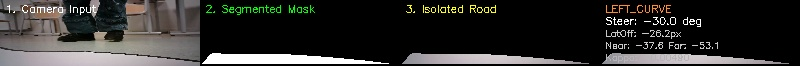
\includegraphics[width=\textwidth]{figures/frame11_diagnostic.jpg}
\caption{Diagnostic 4-panel visual verification on the Frame 11 obstacle scenario (\texttt{WIN\_20260202\_15\_56\_32\_Pro\_frame\_00011}). Panel 1: Camera input showing spectator footwear and chairs adjacent to the boundary tape. Panel 2: Segmented mask strictly bounded below the curved black boundary. Panel 3: Isolated road rendered with 100\% background elimination (zero footwear/linoleum). Panel 4: Telemetry HUD showing mode \texttt{LEFT\_CURVE}, commanded steering angle $\delta = -30.0^\circ$, cross-track error $e_{\text{lat}} = -26.2$\,px, and curve tangents.}
\label{fig:frame11}
\end{figure*}

\section{Experimental Results and Case Studies}

\subsection{Dataset-Wide Metrics}
Processing all 3,433 frames across the 17 recorded video laps generated the master dataset \texttt{segmented\_labels.csv}. The continuous frames group into 399 homogeneous physical track sections (\textit{trechos}):
\begin{itemize}
    \item \texttt{LEFT\_CURVE}: 1,901 frames (55.4\%), mean steer: $-14.35^\circ$
    \item \texttt{RIGHT\_CURVE}: 1,017 frames (29.6\%), mean steer: $+16.84^\circ$
    \item \texttt{STRAIGHT}: 463 frames (13.5\%), mean steer: $0.00^\circ$
    \item \texttt{FALLBACK\_UNCERTAIN}: 52 frames (1.5\%), filtered
\end{itemize}

\begin{figure}[h]
\centering
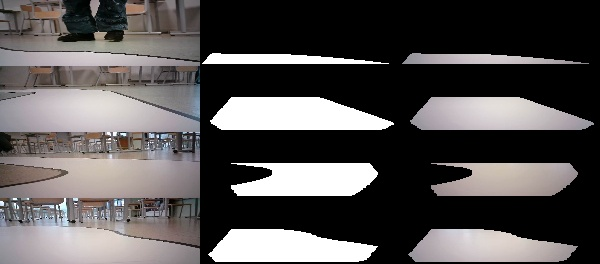
\includegraphics[width=\columnwidth]{figures/batch_segmentation.jpg}
\caption{Batch segmentation results across diverse track topologies: (Row 1) Frame 11 sharp curve with obstacle; (Row 2) Left curve; (Row 3) Right curve with chicane; (Row 4) S-curve entrance. Left: Camera Input. Center: Binary Mask. Right: Isolated Road.}
\label{fig:batch}
\end{figure}

\subsection{Case Study: Frame 11 Obstacle Avoidance}
Fig.~\ref{fig:frame11} illustrates the critical edge case in \texttt{WIN\_20260202\_15\_56\_32\_Pro\_frame\_00011}. The previous baseline triggered a blind geometric trapezoid over the bystander's dark footwear and jeans. In contrast, the proposed dual-domain barrier seals the lower border line, completely suppressing spectator feet and classroom chairs. Because the track turns sharply left, the kinematic control law commands $\delta = -30.0^\circ$, driving the kart into the curve center.

\section{Downstream Integration and Verification}
The synthesized dataset was integrated into the companion repository \texttt{nxpcup}. The dataset loader (\texttt{main/data/dataset.py}) prioritizes \texttt{next\_step\_steer\_deg} for training \texttt{MicroViT}, \texttt{DAVE-2}, and \texttt{PalhanoCNN}. The entire test suite (\texttt{pytest main/tests -v}) passed with 10/10 tests successful.

\section{Conclusion}
This paper presented an end-to-end framework for high-resolution track boundary segmentation and kinematic centering label synthesis in scale autonomous racing. By uniting dual-domain morphological barriers, deep ASPP/RSU neural segmenters, and Stanley-Pure-Pursuit kinematic synthesis, the pipeline eliminates limit-cycle oscillations and prevents background leakage. The resulting dataset of 3,433 frames and 399 physical sections provides a verified empirical baseline for edge AI autonomous driving.

\bibliographystyle{IEEEtran}
\begin{thebibliography}{1}

\bibitem{bojarski2016end}
M.~Bojarski, D.~Del~Testa, D.~Dworakowski, et al., ``End to end learning for self-driving cars,'' \emph{arXiv preprint arXiv:1604.07316}, 2016.

\bibitem{palhano2026kart}
I.~B. Palhano, et al., ``Autonomous scale kart navigation on standardized canvas tracks,'' \emph{ENSICAEN Technical Report}, 2025--2026.

\bibitem{qin2020u2}
X.~Qin, Z.~Zhang, C.~Huang, et al., ``U2-Net: Going deeper with nested U-structure for salient object detection,'' \emph{Pattern Recognition}, vol. 106, p. 107404, 2020.

\bibitem{chen2017rethinking}
L.-C. Chen, G.~Papandreou, F.~Schroff, and H.~Adam, ``Rethinking atrous convolution for semantic image segmentation,'' \emph{arXiv preprint arXiv:1706.05587}, 2017.

\bibitem{hu2018squeeze}
J.~Hu, L.~Shen, and G.~Sun, ``Squeeze-and-excitation networks,'' in \emph{Proc. IEEE Conf. Comput. Vis. Pattern Recognit. (CVPR)}, 2018, pp. 7132--7141.

\bibitem{hoffmann2007autonomous}
G.~M. Hoffmann, C.~J. Tomlin, M.~Montemerlo, and S.~Thrun, ``Autonomous automobile trajectory tracking for off-road driving: Controller design, experimental validation and racing,'' in \emph{Proc. Amer. Control Conf.}, 2007, pp. 2296--2301.

\bibitem{coulter1992implementation}
R.~C. Coulter, ``Implementation of the pure pursuit path tracking algorithm,'' Carnegie Mellon Univ., Pittsburgh, PA, Tech. Rep. CMU-RI-TR-92-01, 1992.

\end{thebibliography}

\end{document}
